\documentclass{article}
\usepackage{graphicx}
\usepackage{makecell}
\usepackage[T1]{fontenc}
\usepackage[dvipsnames]{xcolor}
\usepackage{booktabs}
\usepackage{longtable}
\usepackage{minted}
\usepackage{tgpagella} 
\usepackage{xfrac} 
\usepackage{float} 
\usepackage{colortbl}
\usepackage[most]{tcolorbox}
\RequirePackage{fontawesome}
\usepackage{hyperref}
\hypersetup{
    colorlinks=true, 
    linktoc=all,     
    linkcolor=black!80,
    filecolor=blue,
    urlcolor=cyan!80
}
\usepackage{geometry}
\geometry{a4paper, total={5.5in, 9in}}
\renewcommand{\arraystretch}{1.4}

\tcbset{%
    theoLeft/.style={%
        enhanced,
        breakable,
        sharp corners,
        toprule=1mm, rightrule=0pt, bottomrule=1mm, leftrule=0pt,
        colback=#1!5, colframe=white, coltitle=#1!80!black, 
        detach title,
        overlay unbroken and first ={
            \node[minimum width=1cm, anchor=north west, font=\bfseries] 
               at ([yshift={.4cm}]frame.north west) {\tcbtitle};
        }
    }
}

\definecolor{exampleBox}{RGB}{ 121, 54, 149  }

\newtcbtheorem[auto counter]{code}{}
{theoLeft=exampleBox}{cl}

\title{\huge Architettura e Design}
\author{Gabriele Chignoli}
\date{Giugno 2025}
\begin{document}
\maketitle
\tableofcontents
\newpage

\section{Architettura}
Pantrymanager è un applicativo che prevede l'utilizzo di:
\begin{itemize}
    \item Un'interfaccia grafica per permettere all'utente di interagire con il sistema
    \item Un componente (logica dell'applicazione) che permetta di eseguire operazioni sui dati e fornire un feedback per l'interfaccia
    \item Un componente per conservare una moderata quantità di dati in modo consistente
\end{itemize}
Per questi motivi, lo stile architettonico \textbf{Model-View-Controller (MVC)} è stato scelto come modello più adeguato allo sviluppo dell'applicazione. 

Attraverso il MVC il sistema viene suddiviso in macro-componenti, i quali gestiscono ciascuno una certa funzionalità del software; tale suddivisione consente al sistema un buon grado di modularità, che aiuterà il team sia nelle fasi di sviluppo che in quelle di manutenzione. \newline 

Di seguito viene mostrata la suddivisione prevista dallo stile MVC.  

\begin{itemize}
    \item \textbf{Model} - si occupa di elaborare i dati salvati (e.g. produrre una dieta personalizzata) e gestire la comunicazione con il Database.  
    \item \textbf{View} - mostra all'utente le funzionalità disponibili (e.g. pulsanti per aggiungere/modificare/rimuovere prodotti, creare una dieta personalizzata...), e fornisce l'output del Model all'utente (e.g. i parametri dei vari prodotti, i piatti disponibili...). 
    \item \textbf{Controller} - gestisce gli input dell'utente, fornendo un feedback grafico, e comunica direttamente con il model. 
\end{itemize}

\subsection{Architectural Views}
\subsubsection{Punti di vista del Modulo (Vista Statica)}
\begin{figure}[H]
    \centering
    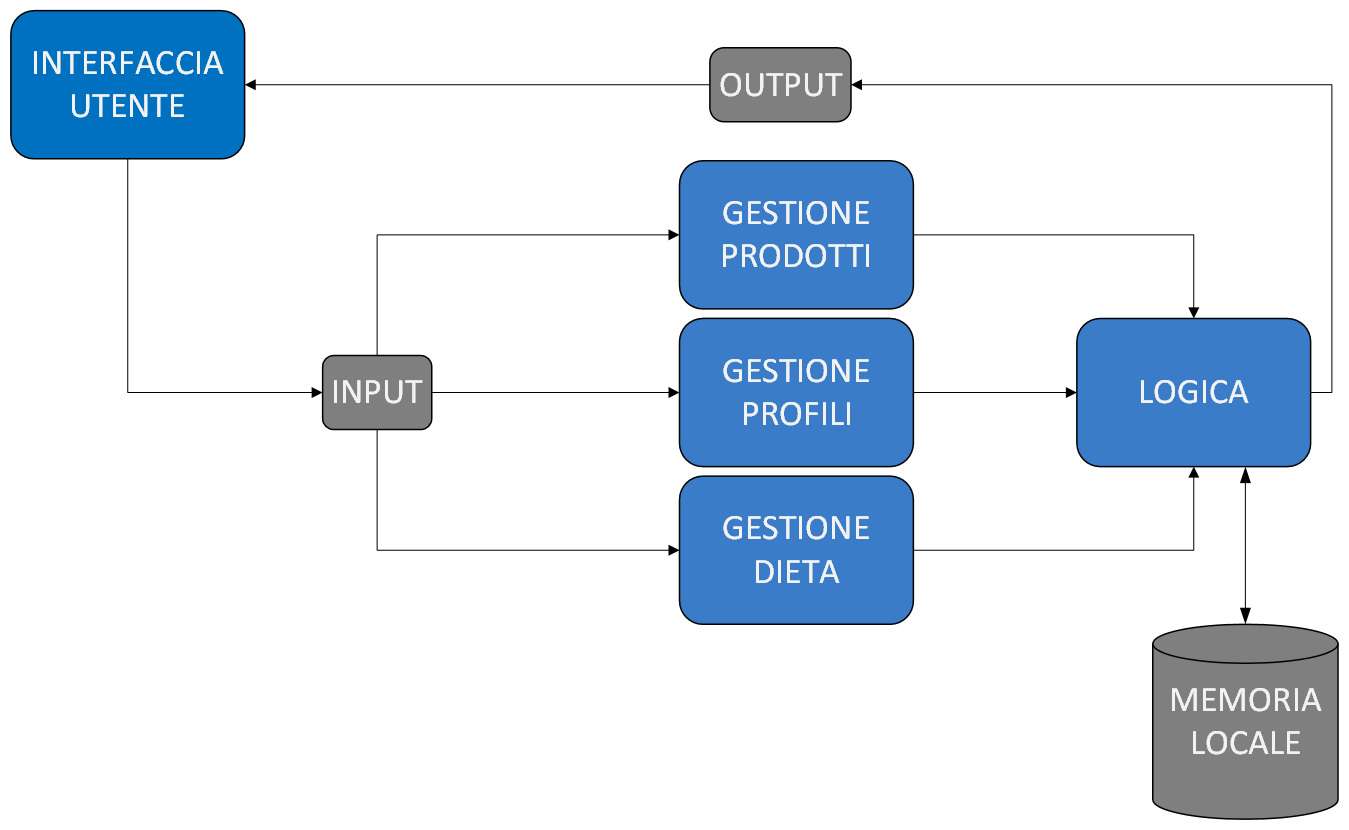
\includegraphics[width=0.8\textwidth]{imgs/VistaModuloUso.png}
    \caption{Punto di vista del modulo con relazione "Usa"}
    \label{fig:enter-label}
\end{figure}
\subsubsection{Punti di vista dei Componenti e dei Connettori (Vista Dinamica)}

\begin{figure}[H]
    \centering
    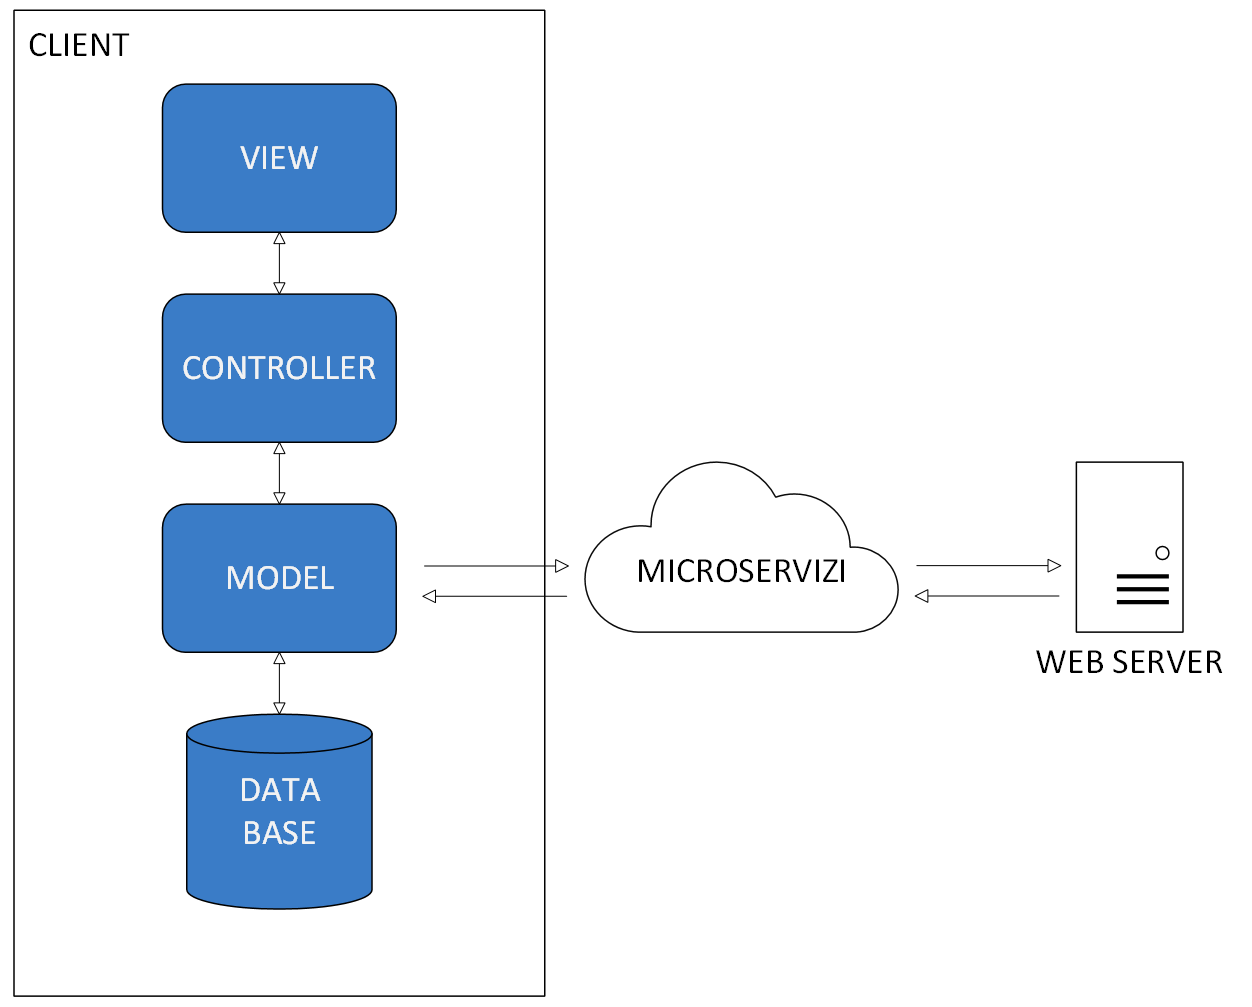
\includegraphics[width=0.8\textwidth]{imgs/Vista.png}
    \caption{Punto di vista dei componenti e dei connettori}
    \label{fig:enter-label}
\end{figure}

La struttura del client è quella che verrà effettivamente sviluppata e utilizzata come riferimento per lo sviluppo del software; i microservizi sono considerati un possibile ampliamento dell'architettura ma che non sarà implementata nella versione finale del software. Inoltre, le relazioni simboleggiate da due frecce distinte in direzione opposta indicano che la relazione è su richiesta, e non un continuo scambio di dati tra i componenti.  
\section{Design}
Viene presentato di seguito il Diagramma delle Classi, volto a mostrare come si intende effettivamente implementare una delle parti costitutive del software. In particolare viene mostrato quali saranno le classi principali, i loro metodi e attributi e le loro relazioni (gerarchia) e interazioni (comunicazione). \newline 

Attraverso Papyrus è possibile generare il codice direttamente dal diagramma UML costruito, tuttavia son stati riscontrati errori (si pensa durante l'installazione) che non permettono il pieno funzionamento dello strumento. Per questo si è deciso di scrivere il codice manualmente utilizzando il diagramma come guida da seguire il più precisamente possibile; si tenterà di tenere aggiornate e coerenti entrambe le versioni.  

\begin{figure}[H]
    \centering
    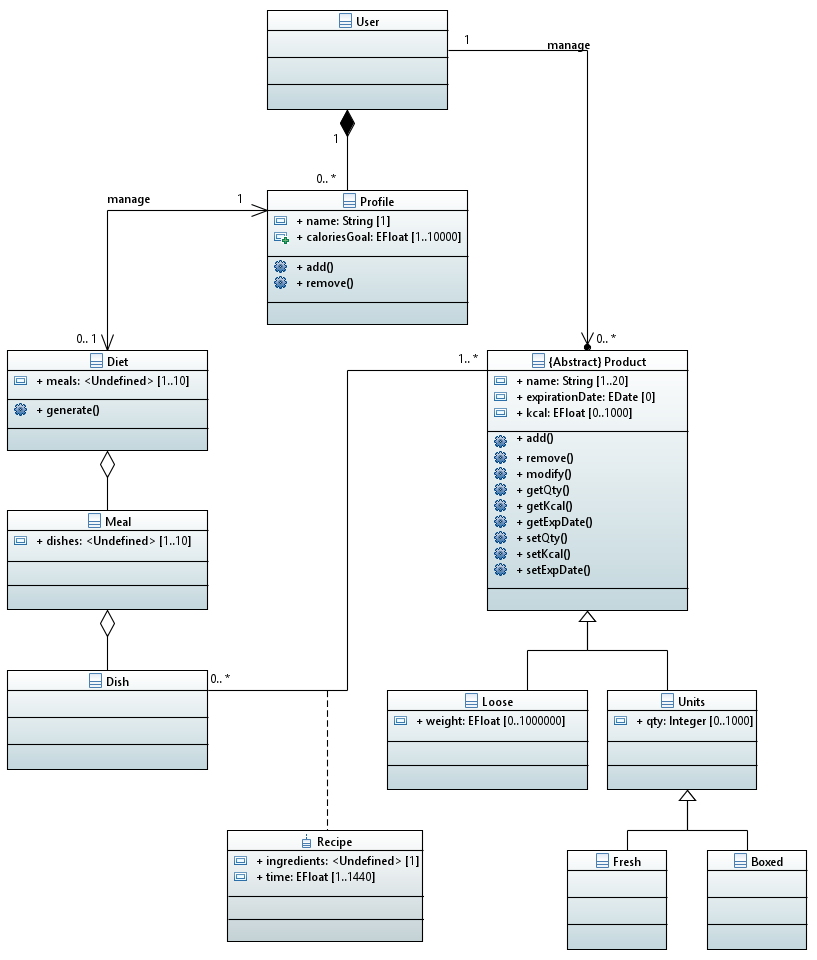
\includegraphics[width=\linewidth]{imgs/ClassDiagram.png}
    \caption{Diagramma delle Classi v0}
    \label{fig:enter-label}
\end{figure}

Si invita il lettore a visionare i diagrammi dalla cartella \texttt{/UML} della documentazione, dove sono disponibili le immagini nelle dimensioni originali.

\begin{figure}[H]
    \centering
    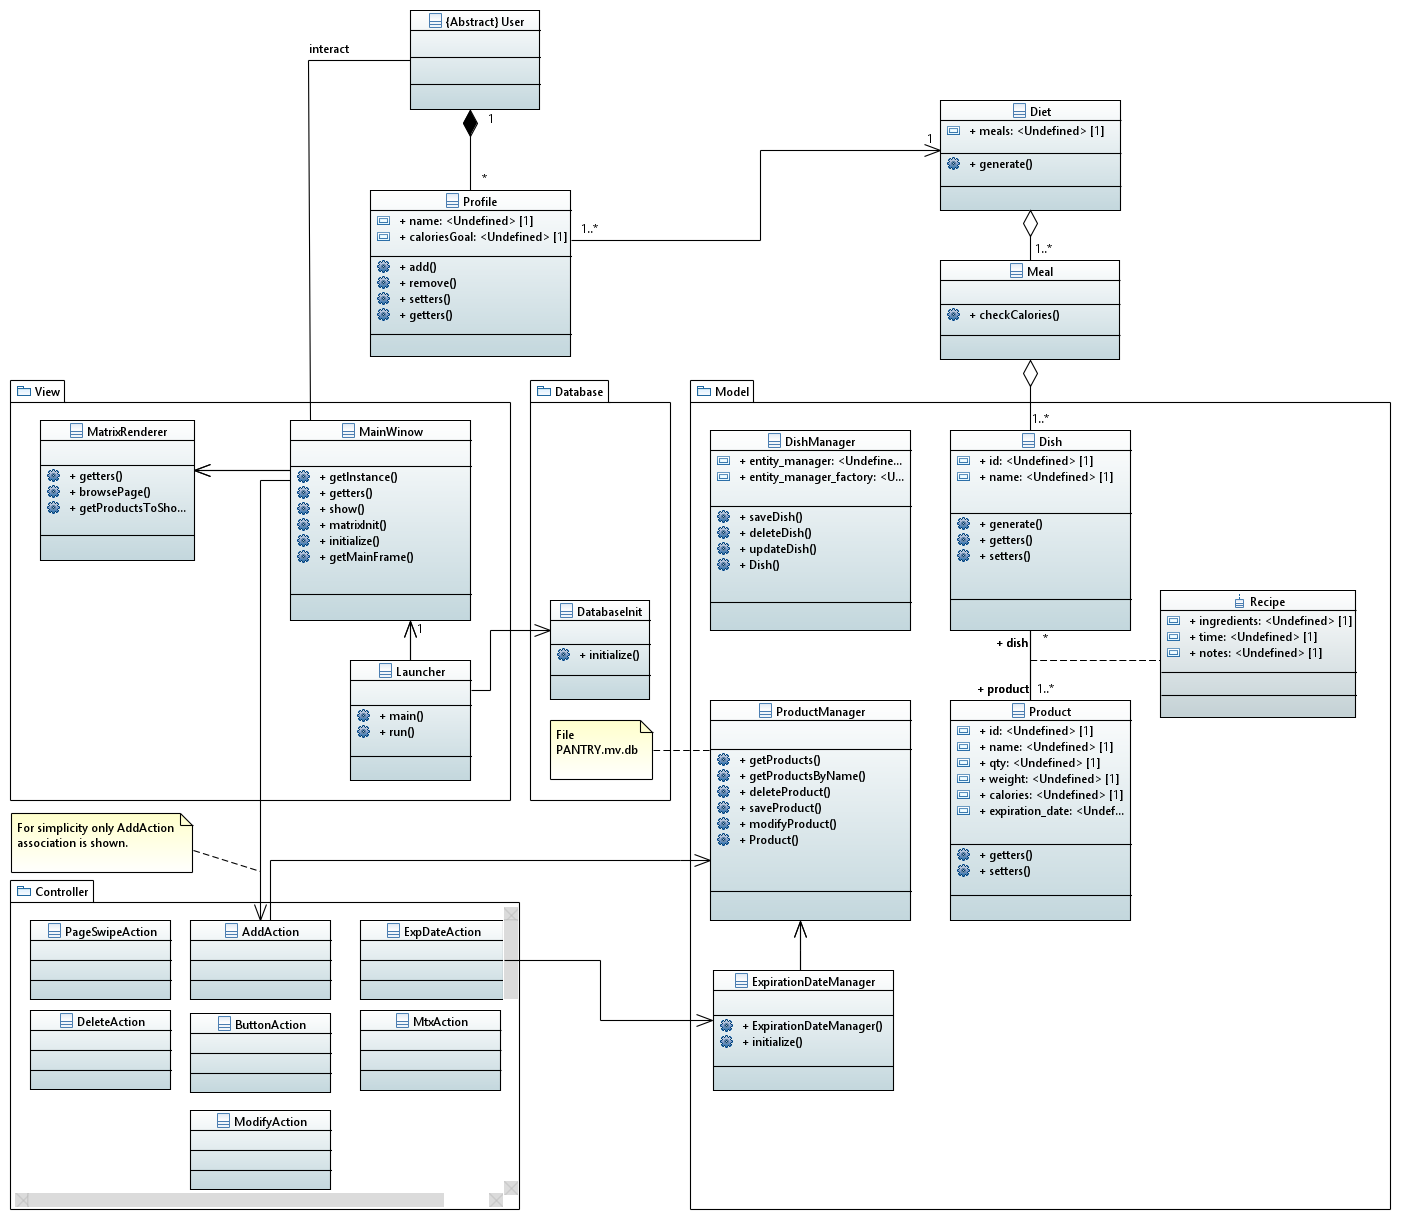
\includegraphics[width=\linewidth]{imgs/ClassDiagram_0.1.0.png}
    \caption{Diagramma delle Classi v1}
    \label{fig:enter-label}
\end{figure}


Viene inoltre presentato il Diagramma delle Componenti (\textit{Figure 5}) al fine di mostrare le interazioni tra le macro-componenti del sistema e le interfacce che questi ultimi devono disporre e utilizzare per garantire il funzionamento dell'applicazione. 
\begin{figure}[H]
    \centering
    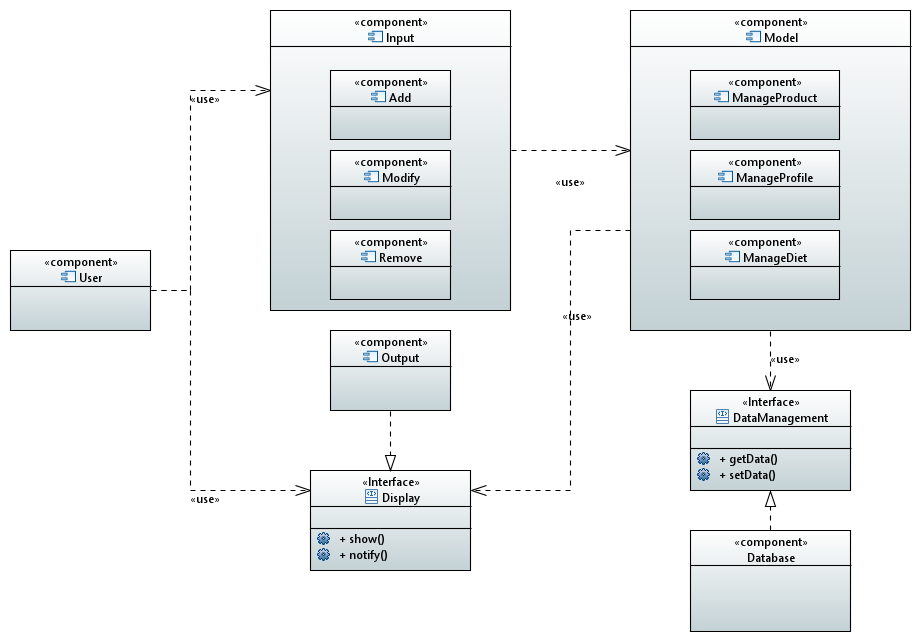
\includegraphics[width=\textwidth]{imgs/ComponentDiagram.png}
    \caption{Component Diagram}
    \label{fig:enter-label}
\end{figure}

\subsection{Gestione dell'interfaccia}
L'interfaccia grafica per l'utente è stata sviluppata utilizzando il framework \textbf{Swing} per Java. Swing permette di costruire finestre e di popolarle con pulsanti, campi e etichette attraverso codice (o utilizzando tool grafici). Il framework prevede che, per garantire l'interazione dell'interfaccia con il resto del sistema, venga utilizzato il \textbf{paradigma degli eventi}: una interazione dell'utente con l'interfaccia grafica genera un evento che viene catturato da delle componenti (detti listener), che in risposta eseguono altro codice. \newline 

In Pantrymanager, ai pulsanti dell'interfaccia (che fa parte del \texttt{package view}) viene assegnata un'azione, il cui evento viene catturato dalle classi listener (contenute nel \texttt{package controller}), che invocano metodi (definiti nelle classi del \texttt{package model}) che agiscono poi effettivamente sui dati in memoria (in lettura e scrittura). \newline 

Come è effettivamente organizzata la struttura può essere osservato direttamente dal folder del progetto, oppure dal diagramma delle classi sopra presentato. 

\subsection{Struttura del Database}
Pantrymanager necessita di avere copie persistenti dei dati su cui deve operare; per raggiungere questo obiettivo si è deciso di utilizzare un \textbf{database embedded, in-memory}, implementato nell'applicativo attraverso il sistema di gestione di database relazionali \textbf{H2}, che permette di creare un database Java SQL.

Per rendere la gestione e la scrittura di codice più semplice, viene integrata la piattaforma \textbf{Hibernate}, un middleware che permette il mapping tra la natura ad oggetti di Java e quella relazionale del database, accoppiata all'interfaccia \textbf{JPA (Jakarta Persistence API)}, che permette la scrittura di query SQL attraverso la notazione puntata della codifica Object Oriented. 

\subsection{Design-Patterns}
\paragraph{Singleton}
La classe \texttt{MainWindow}, che si occupa di generare e popolare la finestra con cui l'utente interagisce, segue il paradigma del \textit{singleton}: è possibile creare una sola istanza della classe, e si accede ad essa solamente attraverso un metodo pubblico che restituisce tale istanza. 

\begin{code*}{}
\begin{minted}{java}
public static MainWindow getInstance() {
    if(instance == null) {
        instance = new MainWindow();
    }
    return instance;
}
\end{minted}
\end{code*}

\subsection{Complessità - \textit{Stan4j}}
Le metriche che vengono presentate in questa sezione sono state estrapolate dal progetto in modo automatico attraverso l'utilizzo del tool \textit{Stan4j}, che permette di eseguire l'analisi statica di un sistema e le sue componenti. 
\subsubsection{Generale}

\begin{figure}[H]
  \centering
  \begin{minipage}{0.4\textwidth}
    \centering
    \includegraphics[width=4cm]{imgs/grafocomplessità.png}
    \caption{Grafo dipendenze progetto}
    \label{fig:enter-label}
  \end{minipage}
  \hfill
  \begin{minipage}{0.4\textwidth}
    \begin{tabular}{lc}
        \toprule
        \textbf{Metrica} & \textbf{Valori} \\
        \midrule
        Cyclomatic Complexity (CC) & \cellcolor{green}1.39  \\
        Fat - Libraries & 1 \\
        Fat - Packages & 6 \\
        Fat - Units & 48 \\
        Tangled & \cellcolor{orange}28.57$\%$ \\
        Distance (D) & \cellcolor{orange}-0.62 \\
        \bottomrule
    \end{tabular}
  \end{minipage}
\end{figure}
\paragraph{Osservazioni}
\begin{itemize}
    \item La complessità è buona (probabilmente dovuto alla semplicità del sistema)
    \item Assente l'utilizzo di classi astratte e interfacce, segnale negativo data la natura ad oggetti di Java
    \item Ci sono dipendenze cicliche nel grafo delle dipendenze
    \begin{itemize}
        \item \texttt{view} e \texttt{model} sono legati da \texttt{ExpirationDateManager.class}, che chiede l'istanza della finestra principale. Si ritiene che sia immediato il fix.
        \item \texttt{view} e \texttt{controller} sono legati da tutte le azioni dei pulsanti. Richiede un'analisi più approfondita.
    \end{itemize}
\end{itemize}

\subsubsection{Model}

\begin{figure}[H]
    \centering
    \includegraphics[width=10cm]{imgs/grafocomplessità_model.png}
    \caption{Grafo dipendenze classi}
    \label{fig:enter-label}
\end{figure}

\begin{figure}[H]
  \centering
  \begin{minipage}{0.4\textwidth}
    \centering
    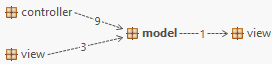
\includegraphics[width=6.5cm]{imgs/coupling_model.png}
    \caption{Grafo dipendenze pacchetti}
    \label{fig:enter-label}
  \end{minipage}
  \hfill
  \begin{minipage}{0.4\textwidth}
    \begin{tabular}{lc}
        \toprule
        \textbf{Metrica} & \textbf{Valori} \\
        \midrule
        Cyclomatic Complexity (CC) & \cellcolor{green}1.28 \\
        Fat & 9 \\
        Afferent Coupling (Ca) & 8 \\
        Efferent Coupling (Ce) & 1 \\
        Instability (I) & \cellcolor{green}0.11 \\
        Abstractness (A) & \cellcolor{red}0 \\
        Distance (D) & \cellcolor{red}-0.89 \\
        \bottomrule
    \end{tabular}
  \end{minipage}
\end{figure}
\paragraph{Osservazioni}
\begin{itemize}
    \item La complessità è buona
    \item La stabilità è soddisfacente, il package dipende poco dagli altri componenti
    \item Assente l'utilizzo di classi astratte e interfacce, segnale negativo data la natura ad oggetti di Java
    \item Distanza troppo alta, il pacchetto è troppo poco astratto
\end{itemize}


\subsubsection{View}

\begin{figure}[h]
    \centering
    \includegraphics[width=5cm]{imgs/grafocomplessità_view.png}
    \caption{Grafo dipendenze classi}
    \label{fig:enter-label}
\end{figure}

\begin{figure}[H]
  \centering
  \begin{minipage}{0.4\textwidth}
    \centering
    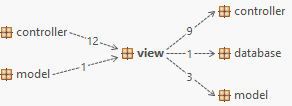
\includegraphics[width=6cm]{imgs/coupling_view.png}
    \caption{Grafo dipendenze pacchetti}
    \label{fig:enter-label}
  \end{minipage}
  \hfill
  \begin{minipage}{0.4\textwidth}
    \begin{tabular}{lc}
        \toprule
        \textbf{Metrica} & \textbf{Valori} \\
        \midrule
        Cyclomatic Complexity (CC) & \cellcolor{green}1.26 \\
        Fat & 4 \\
        Afferent Coupling (Ca) & 9 \\
        Efferent Coupling (Ce) & 12 \\
        Instability (I) & \cellcolor{orange}0.57 \\
        Abstractness (A) & \cellcolor{red}0 \\
        Distance (D) & \cellcolor{orange}-0.43 \\
        \bottomrule
    \end{tabular}
  \end{minipage}
\end{figure}
\paragraph{Osservazioni}
\begin{itemize}
    \item La complessità è buona
    \item L'instabilità richiede attenzione: dal package dipendono molte classi, ma esso stesso ha molte dipendenze
    \item Astrazione assente
    \item Distanza gestibile 
\end{itemize}

\subsubsection{Controller}
\begin{figure}[H]
  \centering
  \begin{minipage}{0.4\textwidth}
    \centering
    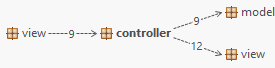
\includegraphics[width=6cm]{imgs/coupling_controller.png}
    \caption{Grafo dipendenze pacchetti}
    \label{fig:enter-label}
  \end{minipage}
  \hfill
  \begin{minipage}{0.4\textwidth}
    \begin{tabular}{lc}
        \toprule
        \textbf{Metrica} & \textbf{Valori} \\
        \midrule
        Cyclomatic Complexity (CC) & \cellcolor{green}1.59 \\
        Fat & 0 \\
        Afferent Coupling (Ca) & 1 \\
        Efferent Coupling (Ce) & 6 \\
        Instability (I) & \cellcolor{red}0.86 \\
        Abstractness (A) &\cellcolor{red} 0 \\
        Distance (D) & \cellcolor{green}-0.14 \\
        \bottomrule
    \end{tabular}
  \end{minipage}
\end{figure}

\paragraph{Osservazioni}
\begin{itemize}
    \item L'instabilità del è troppo alta, il pacchetto non fornisce abbastanza servizi pur dipendendo da molte altre classi (dato dalla natura del pacchetto, in cui sono contenute le azioni dei pulsanti dell'interfaccia)
    \item Astrazione assente
    \item Distanza buona (dovuta all'instabilità molto alta)
\end{itemize}

\subsection{Complessità - \textit{CodeMR}}
\textit{Stan4j} non fornisce per tutte le metriche che calcola dei range per giudicare i valori estrapolati; per questo motivo si è deciso di confrontare i risultati con un altro tool, \textit{CodeMR}, che fornisce un'analisi statica più ampia, graficamente leggibile e soprattutto fornisce un feedback al programmatore più chiaro e diretto. \newline 

Per accedere al report (fornito in formato \texttt{html}), dopo aver scaricato il progetto, aprire il file \texttt{index.html} nella directory
\begin{code*}{}
\texttt{docs/Architettura\_e\_design/codemr/html/main\_report/\dots}
\end{code*}


L'analisi evidenzia una coesione bassa (\textit{medium-high lack of cohesion}) all'interno della classe \texttt{Product}. Si pensa che questo sia dovuto al fatto che si tratta di una classe che serve solo come modello per costruire la struttura del database e per istanziare i prodotti, presentando quindi solamente le variabili necessarie e i metodi getter e setter. 











\end{document}
